\documentclass{standalone}
\usepackage{ tikz }
\usepackage{ xparse }
\usepackage{../../../macros}

\begin{document}
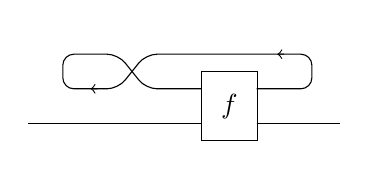
\begin{tikzpicture}[yscale=-1,x=1em,y=1.25em]
    
    \node at (0,-1.5) {};

    \draw (-1,1) -- (5.25,1);

    \draw [rounded corners, ->] (7.25, 0) -- (9.25, 0) -- (9.25,-1) -- (8,-1);
    \draw [rounded corners, ->] (8.25, -1) -- (3.25,-1) -- (2.25, 0) -- (1.25, 0);
    \draw [rounded corners] (1.5,0) -- (0.25,0) -- (0.25,-1) -- (2.25,-1) -- (3.25,0) -- (5.25,0);

    \draw (7.25,1) -- (10.25,1);

    \node[draw, minimum height = 2.5em, minimum width = 2em, anchor = west] at (5.25,0.5){$f$};

\end{tikzpicture}
\end{document}